%\documentclass{beamer}
\documentclass{intbeamer}

% ===== packages =====
\usepackage{etex}
\usepackage[utf8]{inputenc}
\usepackage{graphicx}
\usepackage{tikz}
\usetikzlibrary{positioning, shadows, shapes}
\usepackage{amssymb}



% ===== beamer options =====
\setbeamertemplate{navigation symbols}{}
\graphicspath{{./figs/}}

% ===== titlepage info =====
\title[Towards Open Science in Acoustics]{\huge Towards Open Science \\ in Acoustics \\[.5ex] \normalsize Foundations and best practices}

\author[Spors et al.]{Sascha Spors~$^1$, Matthias Geier~$^1$ and Hagen Wierstorf~$^2$}

\institute[]{$^1$ Institute of Communications Engineering, University of Rostock \\
$^2$ Filmuniversität Babelsberg \emph{KONRAD WOLF}}

\date[7.3.2017]{Jahrestagung der Deutschen Gesellschaft für Akustik \\ 7.3.2017 \\[4ex] 
\includegraphics[scale=.5]{CC_BY4png.png}}

% ===== macros =====
\tikzstyle{box}=[draw=structure.fg!60, fill=structure.fg!50, thick, drop shadow, rounded corners=4pt, minimum width=35mm, minimum height=15mm, anchor=east]
\tikzstyle{box2}=[draw=none, fill=structure.fg!50, thick, rounded corners=0pt, minimum width=35mm, minimum height=10mm, anchor=east]

\newcommand\data[1]{{\color{structure.fg}#1}}

\newcommand\OSstamp[1]{%
\begin{tikzpicture}
\node[box2] (methodology) {#1};
\end{tikzpicture}}

\newcommand\OM{\OSstamp{Open Methodology}}
\newcommand\OS{\OSstamp{Open Source}}
\newcommand\OD{\OSstamp{Open Data}}
\newcommand\OA{\OSstamp{Open Access}}
\newcommand\OPR{\OSstamp{Open Peer Review}}
\newcommand\ONS{\OSstamp{Open Notebook Science}}




% =============================================================================
% =============================================================================
\begin{document}

\maketitle

% =============================================================================
\begin{frame}{The Scientific Method}

\begin{itemize}
\item formulation, testing, and modification of hypotheses
\item systematic observation, measurement, and experiment
\item reproducibility
\end{itemize}

\vfill

\textbf{Branches} {\tiny [Donoho 2009, Stodden 2014a]}
\begin{enumerate}
\item deductive $\rightarrow$ mathematics, formal logic
%
\item empirical $\rightarrow$ statistical analysis of controlled experiments
%
\item computational
\begin{itemize}
\item large-scale simulations
\hspace{16mm}$\smash{\left.\rule{0pt}{.5\dimexpr3\baselineskip+3\itemsep+2\parskip}\right\}
      \text{\parbox{2in}{potentially new branch(es)}}}$
\item data-driven computational science
\end{itemize}
\end{enumerate}

\end{frame}


% =============================================================================
\begin{frame}{Who Should Benefit from my Research?}

\begin{columns}[T]
\begin{column}{.55\linewidth}

\setbeamercovered{invisible}
\begin{itemize}[<+->]
\item[$\square$] myself
\item[$\square$] my future self
\item[$\square$] my colleagues
\item[$\square$] other researchers
\item[$\square$] all people in the world
\item[$\square$] science itself
\end{itemize}

\end{column}
%
\begin{column}{.35\linewidth}

\end{column}
\end{columns}

\end{frame}


% =============================================================================
\begin{frame}{The Elements of Open Science}


\begin{tikzpicture}[node distance=4mm and 4mm]
\node[box] (source) {Open Source};
\node[box, right=of source] (data) {Open Data};
\node[box, right=of data] (access) {Open Access};
\node[box, below=of source] (methodology) {Open Methodology};
\node[box, below=of data] (notebook) {\shortstack{Open Notebook \\ Science}};
\node[box, below=of access] (edu) {\shortstack{Open Educational \\ Resources}};
\node[box, below=of methodology.south east] (review) {Open Peer Review};
\node[box, below=of edu.south west] (reserach) {\shortstack{Open Research}};
\end{tikzpicture}

\vspace{2mm}
{\tiny compiled from \url{https://en.wikipedia.org/wiki/Open_science} and \url{http://openscienceasap.org/open-science}}

\end{frame}


% =============================================================================
\begin{frame}{Example -- Perceptual Study}
\framesubtitle{Procedure}

\begin{columns}[T]
\begin{column}{.41\linewidth}

\begin{enumerate}
\item<1> Idea
\item<2-3> Design of experiment
\item<4-5> Computation
\item<6-7> Experiment
\item<8-9> Analysis
\item<10-11> Manuscript
\item<12-13> Peer review
\item<14-15> Publication
\item<16> Aftermath
\end{enumerate}
\vspace{25mm}

\end{column}
%
\begin{column}{.49\linewidth}

\only<1>{%
\begin{center}

\includegraphics[scale=.20]{./figs/Bright-Idea-800px}
\end{center}

{\tiny \hfill from https://openclipart.org/}
}

\only<2-3>{%
\begin{itemize}
\item hypothesis
\item procedure
\item stimuli
\item test subjects
\item ...
\end{itemize}
}

\only<3>{%
\vspace{2mm}
\begin{center}
\OM
\end{center}
}

\only<4-5>{%
\begin{itemize}
\item mathematical derivations
\item numerical simulations
\item generation of stimuli \\[2ex]
\item control logic, GUI
\end{itemize}
}

\only<5>{%
\vspace{2mm}
\begin{center}
\ONS
\vspace{1mm}
\OD
\vspace{1mm}
\OS
\end{center}
}

\only<6-7>{%
\begin{center}
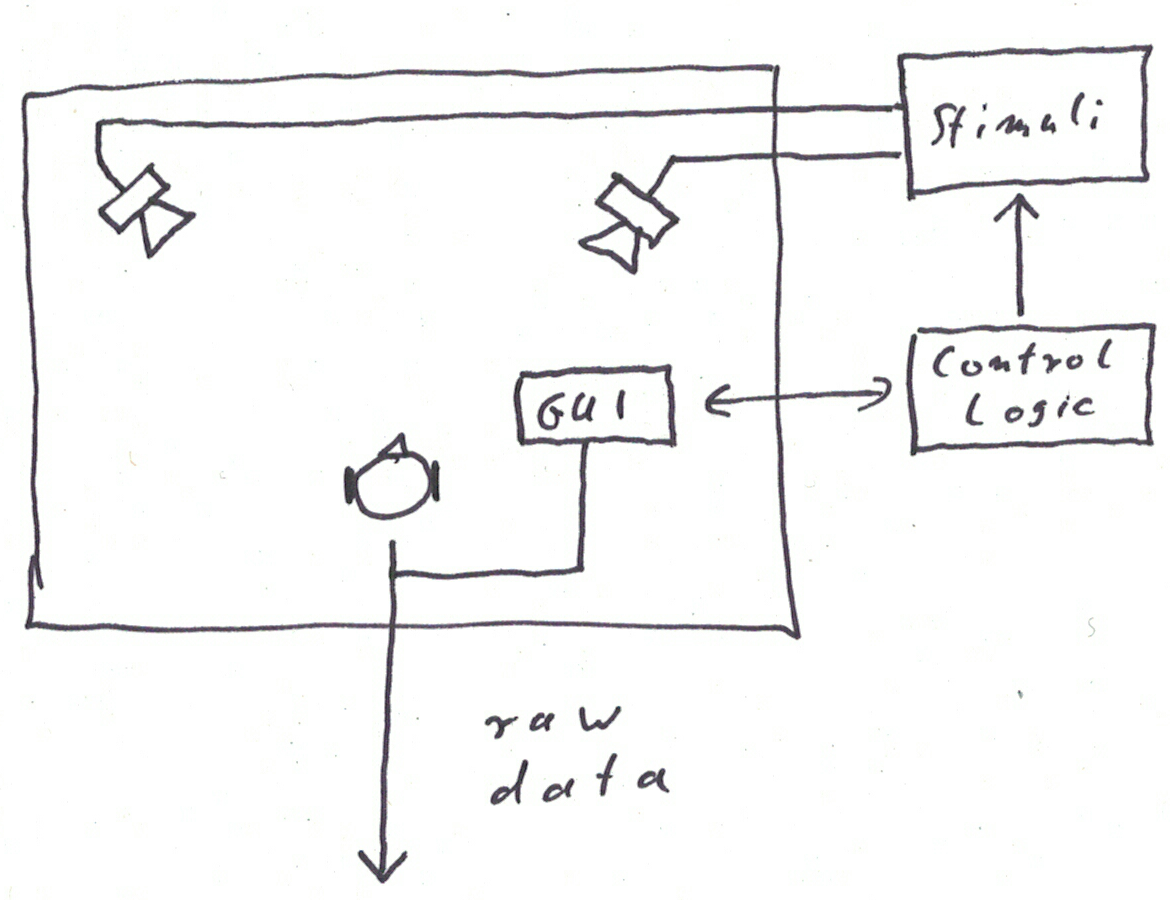
\includegraphics[scale=.13]{experiment}
\end{center}
}

\only<7>{%
\vspace{2mm}
\begin{center}
\OD
\end{center}
}

\only<8-9>{%
\begin{itemize}
\item anonymization of data
\item outlier removal
\item statistical analysis
\end{itemize}
%\textbf{Output:} processed data
}

\only<9>{%
\vspace{2mm}
\begin{center}
\OM
\vspace{2mm}
\OS
\vspace{2mm}
\OD
\end{center}
}

\only<10-11>{%
\begin{itemize}
\item text
\item references
\item visualization of results (plots)
\end{itemize}
}

\only<11>{%
\vspace{2mm}
\begin{center}
\OA
\end{center}
}

\only<12-13>{%
\begin{itemize}
\item ratings, comments
\item revised manuscript
\end{itemize}
}

\only<13>{%
\vspace{2mm}
\begin{center}
\OPR
\end{center}
}

\only<14-15>{%
\begin{itemize}
\item manuscript
\item supplementary materials
\item presentation
\end{itemize}
}

\only<15>{%
\vspace{2mm}
\begin{center}
\OA
\vspace{2mm}
\OS
\vspace{2mm}
\OD
\end{center}
}

\only<16>{%
\begin{itemize}
\item reproduction by third parties
\item post-publication review
\item errata, code and data revision
\item ideas for next study...
\end{itemize}
}
\end{column}
\end{columns}

\end{frame}

% =============================================================================
\begin{frame}{Incentives and Barriers}
\framesubtitle{Selected results from a survey of the machine learning community}

\textbf{Barriers} {\tiny [Stodden 2014], N=134}
\begin{itemize}
\item time to document and clean up (\data{54}/77 \%) \hfill (\data{Data}/Code)
\item dealing with questions from users (\data{34}/52 \%)
\item not receiving attribution (\data{44}/42 \%)
\item possibility of patents (\data{--}/40 \%)
\item legal barriers (e.g. copyright) (\data{34}/41 \%)
\end{itemize}

\vspace{3mm}

\textbf{Incentives}
\begin{itemize}
\item encourage scientific advancement (\data{81}/91 \%)
\item encourage sharing in others (\data{90}/79 \%)
\item be a good community member (\data{86}/79 \%)
\item set a standard in the field (\data{82}/76 \%)
\item improve the calibre of research (\data{85}/74 \%)
\end{itemize}

\end{frame}


% =============================================================================
\begin{frame}{Management of Research Data}

\begin{itemize}
\item systematic management of research data is a prerequisite for open \\ and reproducible science
\item becoming mandatory (DFG, Horizon 2020, NSF, ...)
\end{itemize}

\vfill

\textbf{Principles} {\tiny [DFG 2013, HRK 2014, Stodden 2014b, H2020 2016]}
\begin{itemize}
\item develop a comprehensive data management plan
\item use workflow tracking in the research process
\item make data findable, accessible, interoperable and reusable (FAIR)
\item apply open licensing models
\item offer training and qualification
\end{itemize}

\end{frame}


% =============================================================================
\begin{frame}{Copyright and Licenses}


\begin{itemize}
\item unclear situation when publishing data without explicit license
\item license should be as open as possible to promote re-use
\item legal implications are complex and hard to oversee
\end{itemize}

\vfill

\textbf{Available licensing frameworks}
\begin{itemize}
\item Software: GNU Public License, BSD, MIT, ...
\item Content: Creative Commons, ...
\end{itemize}

\vfill

\textbf{Recommendations}
\begin{itemize}
\item Reproducible Research Standard (RRS) [Stodden, 2009]
\item ...
\end{itemize}

\end{frame}


% =============================================================================
\begin{frame}{Services for Open Science (Selection)}

\begin{columns}[T]
\begin{column}{.45\linewidth}
\textbf{Generic repositories}
\begin{itemize}
\item GitHub
\item Bitbucket
\end{itemize}
\end{column}
%
\begin{column}{.45\linewidth}
\textbf{Repositories for research data}
\begin{itemize}
\item Zenodo
\item runmycode
\item datahub
\end{itemize}
\end{column}
\end{columns}

\vfill

\textbf{Virtual Research Environments}
\begin{itemize}
\item Open Science Framework (OSF)
\item gCUBE
\item hubzero
\end{itemize}

\vfill

\textbf{Journals}
\begin{itemize}
\item Open Science Journal
\item Journal of Open Research Software
\end{itemize}

\end{frame}


% =============================================================================
\begin{frame}{Personal Experience}

\begin{itemize}
\item public release of the SoundScape Renderer (SSR) in 2010
\item various toolboxes, datasets, open access papers, open educational resources
\item internal data management: Redmine, svn, git
\item public releases: github, zenodo, wordpress
\end{itemize}

\vfill

\textbf{Challenges}
\begin{itemize}
\item initial effort (e.g. training)
\item missing versioning tool/platform for (large) data bases
\end{itemize}

\vfill

\textbf{Benefits}
\begin{itemize}
\item documentation/clean up/discussions for public release
\item bug reports, positive community feedback
\item potentially more citations {\tiny [Brody 2006]}
\end{itemize}

\end{frame}


% =============================================================================
\begin{frame}{Conclusions}

\begin{itemize}
\item reproducibility of results is essential for the scientific method
\item Open Science by itself does not ensure the ease of reproducibility
\item evaluation measures contradict scientific innovation
\item training and qualification required
\end{itemize}

\vfill

{\large
\url{https://github.com/spatialaudio}\\[1ex]
\url{https://github.com/twoears}\\[1ex]
\url{http://spatialaudio.net}
}

\end{frame}


% =============================================================================
\begin{frame}{References}

{\scriptsize
\begin{description}
\item[{[Brody 2006]}] T.D. Brody, Evaluating research impact through open access and scholary communication, PhD thesis, May 2006.
\item[{[DFG 2013]}] Sicherung guter wissenschaftlicher Praxis, Deutsche Forschungsgemeinschaft, 2013.
\item[{[Donoho 2009]}] David Donoho, Arian Maleki, Inam Rahman, Morteza Shahram, Victoria Stodden, 15 Years of Reproducible Research in Computational Harmonic Analysis, Computing in Science and Engineering, 11(1), 2009.
\item[{[HRK 2014]}] Hochschulrektorenkonferenz. Management von Forschungsdaten - eine zentrale strategische Herausforderung für Hochschulleitungen, 13.5.2014.
\item[{[H2020 2016]}] H2020 Programme: Guidelines of FAIR Data Management in Horizon 2020, European Research Commission, 26.7.2016.
\item[{[Stodden 2009]}] Vitoria Stodden, The Legal Framework for Reproducible Scientific Research, Computing in Science \& Engineering, January/February 2009.
\item[{[Stodden 2014a]}] Victoria Stodden, Resolving Reproducibility in Computational Science: Tools, Policy, and Culture, talk, 8.10.2014.
\item[{[Stodden 2014b]}] Victoria Stodden and Sheila Miguez, Best Practices for Computational Science: Software Infrastructure and Environments for Reproducible and Extensible Research, Journal of Open Reserach Software, 2(1):e21, pp. 1-6.


\end{description}
}

\end{frame}


\end{document}